\documentclass{article}
\usepackage{amsmath}
\usepackage{amssymb}
\usepackage{graphicx}
\usepackage{hyperref}
\usepackage[version=4]{mhchem}


\begin{document}
\section*{Problem}
A circle is inscribed in triangle \(A B C\). The tangent points are \(D, E, F\) as shown. Show that \(\angle F D E=90^{\circ}-\frac{1}{2} \angle A\).\\
\centering
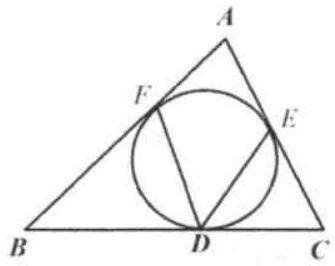
\includegraphics[width=\textwidth]{images/154(1).jpg}

\section*{Solution}
Connect \(O E, O F\).\\
Since both \(A F\) and \(A E\) are tangent to circle \(O, A F \perp O F, A E \perp O E, \angle A F O=\) \(\angle A E O=90^{\circ}\).

In quadrilateral \(\mathrm{AFOE}, \angle A+\angle F O E=360^{\circ}-2 \times 90^{\circ}\) \(=180^{\circ}\).

So \(\angle F O E=180^{\circ}-\angle A\)\\
But \(\angle F D E=\frac{1}{2} \angle F O E\). So \(\angle F D E=90^{\circ}-\frac{1}{2} \angle A\).\\
\centering
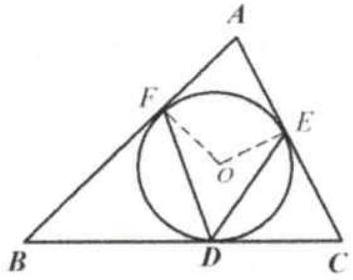
\includegraphics[width=\textwidth]{images/157(2).jpg}

\end{document}
